\documentclass{article}
\usepackage{graphicx}
\usepackage{amsmath}% http://ctan.org/pkg/amsmath
\usepackage{kbordermatrix}% http://www.hss.caltech.edu/~kcb/TeX/kbordermatrix.sty

\usepackage[L7x,T2A]{fontenc}
\usepackage[utf8]{inputenc}
\usepackage[lithuanian]{babel}

\usepackage{breqn}
\usepackage{mathtools,hyperref}
\usepackage{float}







\usepackage{caption}

\usepackage{subcaption}

\begin{document}

\title{Natural Language Processing for Lithuanian language}
\author{Mindaugas Venckus}

\maketitle

\begin{abstract}
Main intention of this research is to study and learn natural language processing (NLP) principals  for Lithuanian language. It is interesting to implement classical nlp methods and see how they work on it. In this work text classification, topics extraction, search query, clustering ideas were implemented.
\end{abstract}

\section{Data}
Data analysis can't be established without having textual data, due to my work started from getting raw data from most popular news website www.delfi.lt. I decided to crawl articles from 5 categories (Criminals, Music, Movies, Sports, Science) such approach helps me to understand better the performance of NLP methods. Below is presented basic statistics of data we analysed  \ref{DocumentsTable}.
\begin{table}[htb]
\centering
\caption{Documents}
\label{DocumentsTable}
\begin{tabular}{|l|l|}
\hline
          & documents count \\ \hline
criminals & 227             \\ \hline
movies    & 167             \\ \hline
music     & 120             \\ \hline
science   & 204             \\ \hline
sports    & 136             \\ \hline
\end{tabular}
\end{table}
\section{Preprocessing}
 
We need to convert unstructured data (raw text) to structured (matrix based approach) such transformation is friendly for machine learning algorithms. So my preprocessing goal is to convert unstructured data to  structured matrix where rows - document id, columns - token, values - term frequency inverse document frequency (tfidf).


\renewcommand{\kbldelim}{(}% Left delimiter
\renewcommand{\kbrdelim}{)}% Right delimiter
\[
  \text{tfidf\_matrix} = \kbordermatrix{
    & token_1 & token_2 & token_3 & . & token_n \\
    doc_1 & 0 & 0 &  & . & 0 \\
    doc_2 & 0 &  & 0.14 & . & 0 \\
    doc_3 & 0 & 0 & 0 & . & 0 \\
    . & . & . & . & . & . \\
    doc_n & 0 & 0.011 & 0 & . & 0
  }
\]

\subsection{Tokenization}
Suppose we have raw text bellow: \\
\textsc{Pranešimas gautas apie 14.14 val. Kaune, Švenčionių g. prie Nemuno upės ant kranto rastas žmogaus kūnas su galimai durtine žaizda krūtinėje. Aplinkybės tikslinamos.}
Tokenization is the process of breaking a text into smaller words, phrases, symbols. In our cases we are trying to break text into the words.

\begin{enumerate}
\item  Break text into the words using regex expression \text{W+} which breaks text by any non-word character.
\begin{enumerate}
\item Remove digits
\item Remove words smaller than 4 letters
\item Remove stop words (unnecessary/common words)
\item Remove word endings
\end{enumerate}
\end{enumerate}
Text above is transformed to list representation
\textsc{t = [aplinkyb, durtin, gaut, kaun, krant, krūtin, kūn, nemun, praneš, rast, tikslinam, up ,švenčion, žaizd, žmog]}


\subsection{tfidf}
tfidf \ref{tfidf} is statistic which measure token importance in document with relation to the document of corpus.
\begin{equation}
\label{tfidf}
tfidf(t, d, D) = tf(t, d) \cdot  idf(t,D)
\end{equation}

where term frequency $ tf(t, d)$ - is a measure of how many times token $t$ occurs in the document $d$ and inverse document frequency $idf(t, D) $ is a measure of how much information the word provides, that is, whether the term is common or rare across all documents.
\begin{equation}
idf(t, D) = \log \frac{N}{|d\in D : t \in d|}
\label{idf}
\end{equation}
with 
\begin{enumerate}
\item $N$ - total number of documents in corpus $N = |D|$
\item $|d\in D : t \in d|$ - number of documents where term $t$ appears.
\end{enumerate}
tfidf intuitive explanation -  importance increases proportionally to the number of times a word appears in the document but is offset by the frequency of the word in the corpus.

\subsection{tfidf matrix construction}
Main steps before matrix construction are:
\begin{enumerate}
\item For each document $90\%$ - train set, $10\%$ - test set.
\begin{enumerate}
\item Collect tokens for each document separately.
\item Collect unique tokens.
\item Collect document categories (will be used for classification performance measuring)
\item Collect document titles(will be used for clustering)
\end{enumerate}
\end{enumerate}

Construct zeros matrix where rows are all documents and columns unique tokens. Fill matrix values with tfidf statistic. Additionally we reduce matrix dimension by removing tokens (entire column) which appears rarely among documents, more precisely  once a time.
\section{Classification}
Main idea of classification is to convert unseen text to vectorized token representations where tokens are taken from tfidf matrix and do multiplication between vector and mentioned matrix. After that use k-nearest approach to make prediction for unseen document by taking mode of most similar $k$ documents categories.


\subsection{Classification results}
Classification performance is measured using confusion matrix where rows are true category and columns predicted category. As we see from figure \ref{confusion matrix} We tried to predict category for 13 movies and got 1 criminals, 1 sports , 11 movies prediction. In overall such approach reach above $90 \%$  recall and $90 \%$ precision.
\begin{figure}[H]
  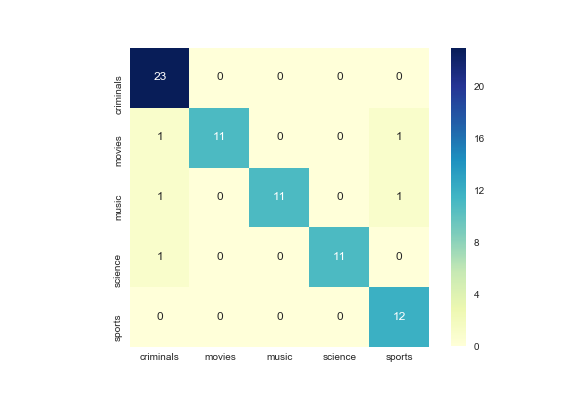
\includegraphics[width=\linewidth]{images/confussion_matrix.png}
  \caption{Classification performance}
  \label{confusion matrix}
\end{figure}


\end{document}